% Made up for the tikra benchmark.
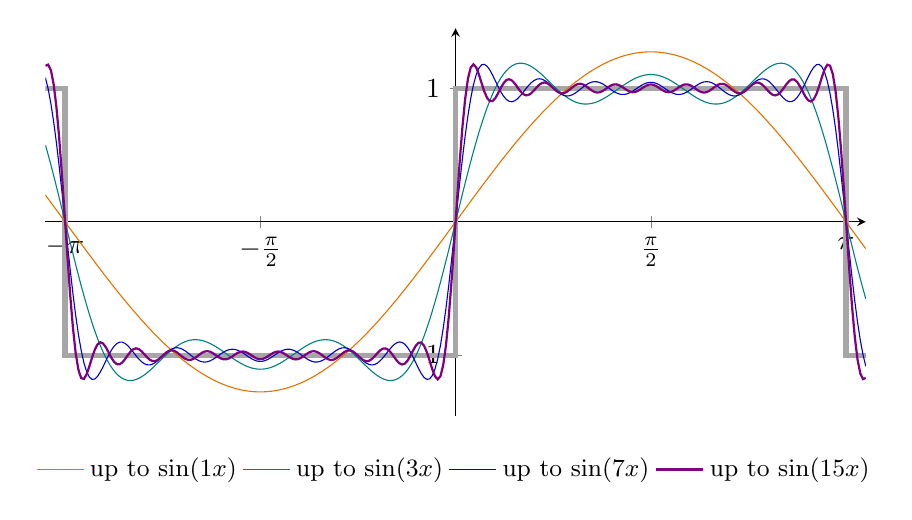
\begin{tikzpicture}
\begin{axis}[width=12cm, height=6.5cm, xmin=-3.3, xmax=3.3, ymin=-1.45, ymax=1.45,
    axis lines=middle, xtick={-3.1416,-1.5708,1.5708,3.1416},
    xticklabels={$-\pi$,$-\frac{\pi}{2}$,$\frac{\pi}{2}$,$\pi$}, ytick={-1,1},
    samples=300, domain=-3.3:3.3, legend style={at={(0.5,-0.08)}, anchor=north, legend columns=4,
    draw=none, font=\small}, cycle list={{orange!90!black}, {teal}, {blue!80!black}, {violet, thick}}]
  \addplot[black!35, line width=2pt, const plot, forget plot]
    coordinates {(-3.3,1) (-3.1416,-1) (0,1) (3.1416,-1) (3.3,-1)};
  \pgfplotsinvokeforeach{1,3,7,15}{
    \addplot+[no marks] {4/pi*sin(deg(x))
      + (#1>=3)*4/(3*pi)*sin(deg(3*x)) + (#1>=3)*4/(5*pi)*sin(deg(5*x))
      + (#1>=7)*4/(7*pi)*sin(deg(7*x)) + (#1>=7)*4/(9*pi)*sin(deg(9*x))
      + (#1>=7)*4/(11*pi)*sin(deg(11*x)) + (#1>=7)*4/(13*pi)*sin(deg(13*x))
      + (#1>=15)*4/(15*pi)*sin(deg(15*x)) + (#1>=15)*4/(17*pi)*sin(deg(17*x))
      + (#1>=15)*4/(19*pi)*sin(deg(19*x)) + (#1>=15)*4/(21*pi)*sin(deg(21*x))};
    \addlegendentry{up to $\sin(#1 x)$}
  }
\end{axis}
\end{tikzpicture}
